%!TEX root = ../thesis.tex

\chapter{Results}
\label{ch:results}

\section{Exploring the Data: Cluster Analysis}

In order to better understand the player profiles, I used the $k$-means clustering
algorithm to separate player-seasons into clusters based on their tendencies. This
algorithm works by adjusting cluster centers in order to minimize inertia, also
known as within-cluster sum of squares:
$$
\sum_{i=1}^n \min_{c \in C} \lVert x_i - \mu_c \rVert^2
$$
where $C$ is the set of clusters and $\mu_c$ is the center of cluster $c$. The
$k$-means algorithm was chosen over other clustering algorithms for a few reasons;
first, it is a simple and easy-to-understand algorithm that often gives intuitive
results and has few parameters to tune other than the number of clusters. Second,
using inertia as the loss function for clustering assumes that clusters are convex
and isotropic, which is a reasonable assumption for player types; in other words,
the shapes of a cluster of players in player profile space should be roughly
spherical, rather than elongated.

In order to apply $k$-means to the player profiles, I used player profile data from
every season from 2006-07 to 2015-16, ignoring the ``replacement player'' category
used for the regression analysis so that the 360 players involved in the most plays
in each season were considered. As noted in section~\ref{sec:profiles}, the profiles
were normalized within each year by subtracting a given season's average for each
feature and dividing by its standard deviation; this is necessary because $k$-means
treats each datum as a point in space, so it is necessary for each feature to be on
the same scale.

Next, because $k$-means weights each dimension equally in computing distances, steps
must be taken to ensure that the many offensive features do not dominate the
relatively few defensive and rebounding features when distances are computed in
$k$-means. To remedy this problem, the variances of the five defensive and two
rebounding features were inflated by factors of 2 and 3 respectively so that they
are not drowned out by variance from the 25 offensive features. While these
adjustments were ad-hoc, they yielded intuitive results; moreover, the fact that
defensive and rebounding features are correlated with some offensive features
ensures that some of this signal is encapsulated in the offensive features. For
example, both rebounding features were heavily correlated with the proportion of ap
layer's shots taken from within four feet of the basket, as was block rate;
similarly, steal rate is correlated with a player's field goal percentage on corner
three-point attempts.

In order to determine the optimal number of clusters $k$, the goodness of fit for
a given value of $k$ was determined by the average silhouette score over all data
points. The silhouette score for a data point $x_i$ assigned to cluster $c$ of $N_c$
points is given by
$$
\frac{b_i - a_i}{\max(a_i, b_i)}
$$
where $a_i$ is the average distance between $x_i$ and all other points in cluster
$c$ and $b_i$ is the smallest average distance between $x_i$ and the nearest cluster
to which $x_i$ does not belong:
$$
a_i = \frac{1}{N_c} \sum_{x_j \in c} \lVert x_i - x_j \rVert \qquad
b_i = \min_{c' \neq c} \frac{1}{N_{c'}} \sum_{x_j \in c'} \lVert x_i - x_j
\rVert
$$
Therefore, a silhouette score close to one indicates that the point is
well-clustered, whereas a score close to zero indicates that a point is near the
border between clusters. Thus, a good clustering will have a higher average
silhouette score than a worse clustering. The average silhouette scores for various
values of $k$ are shown in figure~\ref{fig:sils}.

\begin{figure}
    \centering
    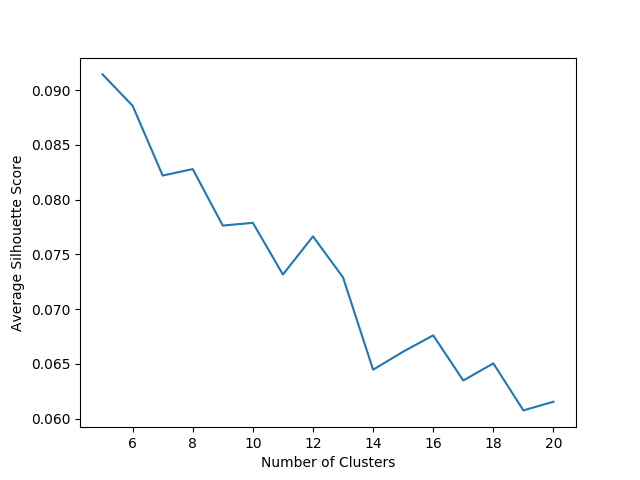
\includegraphics[width=0.75\textwidth]{figures/sil_scores}
    \caption{Average silhouette scores for various values of $k$.}
    \label{fig:sils}
\end{figure}

From this figure, $k=8$ was chosen to be the best choice for the number of clusters.
This is because there is a relatively large dropoff after $k=8$, whereas there
is actually an increase in average silhouette scores from $k=7$ to $k=8$; moreover,
while there are greater average silhouette scores for lower values of $k$, these
values are so low that the clusters would not be as interesting. For example, if
$k=5$ was chosen, then the clusters would probably have a high correlation with
the five traditional positions in basketball and thus the clustering would provide
little insight.

After re-applying the $k$-means algorithm with $k=8$, we arrive at cluster means as
shown in figure~\ref{tab:clus_means}. Note that the means shown are the means of the
data that is after standardization by year but prior to inflating the variance of
the defense and rebounding features.

\begin{table}
    \centering
    \noindent\makebox[\textwidth]{%
\begin{tabular}{ccccccccc}
\toprule
    & \multicolumn{8}{c}{Cluster} \\
Feature &     1 &     2 &     3 &     4 &     5 &     6 &     7 &     8 \\
\midrule
FGA per play                   & -0.28 & -0.65 &  0.38 &  0.22 &  0.59 &  0.53 & -0.29 & -1.03\\
AST per teammate FGM           & -0.40 & -0.83 & -0.34 &  0.98 & -0.36 &  1.09 & -0.50 & -0.82 \\
FT \%                          &  0.36 & -0.67 &  0.12 &  0.20 & -0.04 &  0.62 & -0.37 & -1.42 \\
FTA per FGA                    & -0.76 &  0.55 & -0.14 & -0.03 &  0.19 & -0.23 &  0.10 &  1.47\\
PF drawn per play              & -0.89 &  0.12 &  0.03 &  0.21 &  0.66 &  0.11 & -0.08 &  0.55\\
Lost balls per play            & -0.77 & -0.03 & -0.00 &  0.36 &  0.49 &  0.40 & -0.21 & -0.08\\
Bad passes per play            & -0.39 & -0.79 & -0.29 &  0.96 & -0.32 &  0.88 & -0.33 & -0.71\\
Travels per play               & -0.41 &  0.31 &  0.13 & -0.13 &  0.52 & -0.16 &  0.24 &  0.12 \\
Offensive fouls per play       & -0.66 &  1.06 &  0.01 & -0.24 &  0.35 & -0.43 &  0.29 &  0.85\\
Percent of 2-pt FGM assisted   &  0.32 &  0.79 &  0.31 & -0.86 &  0.56 & -1.12 &  0.67 &  0.56\\
Percent of 3-pt FGM assisted   &  0.65 & -1.42 &  0.59 &  0.27 & -0.40 &  0.21 &  0.33 & -1.56\\
Percent of FGA, 2-pt $\leq$ 4 ft & -0.86 &  0.89 & -0.23 & -0.19 &  0.35 & -0.52 &  0.29 &  1.95 \\
Percent of FGA, 2-pt 5-8 ft    & -0.74 &  1.05 & -0.08 & -0.34 &  0.91 & -0.30 & -0.02 &  0.86\\
Percent of FGA, 2-pt 9-16 ft   & -0.54 &  0.53 &  0.08 & -0.15 &  0.95 &  0.14 &  0.00 & -0.56\\
Percent of FGA, 2-pt 17+ ft    &  0.08 & -0.40 &  0.20 &  0.09 &  0.07 &  0.34 &  0.29 & -1.29 \\
Percent of FGA, 3-pt $\leq$ 23 ft &  1.33 & -0.82 &  0.02 &  0.04 & -0.76 & -0.06 & -0.23 & -0.86 \\
Percent of FGA, 3-pt 24-26 ft  &  1.06 & -1.09 &  0.13 &  0.30 & -0.95 &  0.37 & -0.41 & -1.13 \\
Percent of FGA, 3-pt 27-30 ft  &  0.54 & -0.82 & -0.02 &  0.30 & -0.72 &  0.56 & -0.35 & -0.82 \\
FG\%, 2-pt $\leq$ 4 ft         & -0.20 &  0.30 &  0.20 & -0.20 &  0.47 & -0.38 &  0.14 &  0.31 \\
FG\%, 2-pt 5-8 ft              & -0.18 &  0.18 &  0.15 & -0.12 &  0.37 &  0.10 & -0.23 & -0.16\\
FG\%, 2-pt 9-16 ft             &  0.04 & -0.04 &  0.02 & -0.06 &  0.25 &  0.22 & -0.16 & -0.53\\
FG\%, 2-pt 17+ ft              &  0.13 & -0.10 &  0.14 &  0.07 &  0.21 &  0.24 & -0.02 & -1.21 \\
FG\%, 3-pt $\leq$ 23 ft        &  0.51 & -1.08 &  0.32 &  0.31 & -0.69 &  0.47 & -0.06 & -1.16 \\
FG\%, 3-pt 24-26 ft            &  0.53 & -1.32 &  0.33 &  0.33 & -0.48 &  0.50 & -0.05 & -1.25 \\
FG\%, 3-pt 27-30 ft            &  0.39 & -0.76 &  0.25 &  0.26 & -0.40 &  0.35 & -0.22 & -0.90 \\
Blocks per opponent 2-pt FGA   & -0.51 &  1.26 & -0.13 & -0.52 &  0.68 & -0.75 &  0.29 &  1.37 \\
Steals per play                & -0.24 & -0.79 & -0.46 &  1.48 & -0.51 & -0.02 &  0.31 & -0.29 \\
Personal fouls per play        & -0.34 &  1.39 & -0.28 & -0.37 & -0.03 & -0.70 &  0.61 &  1.03 \\
Opponent TO per play           & -0.07 & -0.30 & -0.46 &  0.81 & -0.46 & -0.48 &  0.94 &  0.18\\
Offensive rebounding rate      & -0.75 &  1.11 & -0.08 & -0.64 &  1.08 & -0.88 &  0.49 &  1.84 \\
Defensive rebounding rate      & -0.65 &  0.47 &  0.24 & -0.58 &  1.59 & -0.95 &  0.42 &  1.48 \\
Defensive RAPM                 &  0.03 & -0.10 & -0.43 &  0.51 & -0.01 & -0.63 &  0.60 &  0.50 \\
Offensive RAPM                 & -0.03 & -0.48 &  0.12 &  0.17 &  0.18 &  0.18 & -0.21 & -0.16 \\
\bottomrule
\end{tabular}
    }
    \caption{Player profile for the average member of each cluster.}
    \label{tab:clus_means}
\end{table}

TODO: finish this

Many of these clusters intuitively describe player types in the NBA. For example,
cluster 1 seems to represent three-point specialists, or players who don't shoot
often but shoot most of their shots from three-point range, and are successful from
that range; these players often make their shots 

Cluster 1: 3-pt specialist
Cluster 2: low-usage big man with poor offense
Cluster 3: average all-around wing
Cluster 4: 

\section{Cross-Validation Results}

As explained in section~\ref{sec:mod_sel}, cross-validation was done using three
randomly selected seasons on each run; many different cross-validation runs were
done in order to tune model hyperparameters; the results are summarized in
table~\ref{tab:cv_results}.

\begin{table}
    \centering
    \noindent\makebox[\textwidth]{%
    \begin{tabular}{cc|ccc}
        \toprule
        & Optimal Hyperparameters &
        Linear Regression & Random Forests & Gradient-Boosting \\[1em]
        Optimal Hyperparameters & & N/A & \parbox[c]{3cm}{300 estimators,\\ max
        depth 3} & \parbox[c]{3cm}{300 estimators,\\ max depth 3,\\ learning
        rate 0.1} \\ \midrule
        PCA & \parbox[c]{3cm}{5 components} & 1.263605* & 1.264270 &
        1.264506 \\ \midrule
        Isomap & \parbox[c]{3cm}{5 components,\\ 5 neighbors} & 1.266315 &
        1.266019 & 1.267266 \\ \midrule
        LLE & \parbox[c]{3cm}{5 components,\\ 5 neighbors} & 1.266406 & 1.266016 &
        1.267420 \\
        \bottomrule
    \end{tabular}
    }
    \caption{A summary of the results of hyperparameter tuning and
    cross-validation.}
    \label{tab:cv_results}
\end{table}

Somewhat surprisingly, the regression model with the best performance in
cross-validation is the simple linear regression model. Moreover, less surprisingly,
principal components analysis beat out the nonlinear dimensionality reduction
techniques, as models trained using PCA outperformed Isomap and LLE regardless of
the regression model used. As noted in section~\ref{sec:regress}, the linear
regression model does encapsulate interactions between players, to an extent; this
is because the players are sorted in order of total RAPM, so unlike the baseline
RAPM model discussed in the introduction and in section~\ref{sec:baseline},
substituting player 1 for player 2 is not as simple as adding one player 1's ratings
and subtracting player 2's ratings because the substitution can result in a
shuffling of the order of the players in the regression, which in turn means that
a player's feature values may be matched with different coefficients if his position
in the sorted lineup changes as a result of the substitution. Therefore, while it is
not a nonlinear model, this linear regression model still functions differently than
the adjusted plus/minus model in that the effect of a substitution is not
necessarily the same regardless of the other players on the court as it is in the
APM model.

\section{Comparison to Baseline Model}
\label{sec:baseline}

The motivation for this model is to incorporate play styles in order to improve upon
the regularized adjusted plus/minus model when predicting the relative performance
of two lineups. However, the (R)APM framework is used as a method for evaluating
individual players and is not used to produce predictions for two arbitrary lineups;
therefore, an extension of the model is necessary in order to adapt it to
predict the outcome of a possession. If one is to accept the RAPM model's assumption
that the point outcome of a possession can be linearly allocated to the ten players
on the court as in~\eqref{eq:apm}, then it naturally follows from the model to model
the points per possession of one lineup against another as a linear combination of
the players' RAPM ratings with a home court adjustment:
\begin{equation} \label{eqn:baseline}
    y_i = \sum_{p \in OP_i} x_{\text{off}, p} - \sum_{p \in DP_i} x_{\text{def}, p}
    + \beta_{\text{HCA}}x_{\text{HmOff},i} + \beta_{\text{const}} + \epsilon_i
\end{equation}
where $y_i$ represents points on a possession $i$, $OP_i$ and $DP_i$ are the sets of
offensive and defensive players on the court for possession $i$ respectively,
$x_{\text{off}, p}$ and $x_{\text{def}, p}$ are player $p$'s computed ORAPM and
DRAPM ratings respectively, $x_{\text{HmOff}, i}$ is an indicator for whether the
home team is on offense for possession $i$, and $\epsilon_i$ is a
normally-distributed error term with zero mean. Then, the coefficients
$\beta_{\text{HCA}}$ and $\beta_{\text{const}}$ are optimized via ordinary least
squares. Note that the ORAPM and DRAPM predictors are not given coefficients; this
is because the RAPM model inherently assumes that these ratings combine linearly
with equal weights for each player. This assumption is made by the APM model
in~\eqref{eq:apm} wherein points on a possession is modeled as equal to the sum of
the offensive players' coefficients minus the sum of the defensive players'
coefficients, using an indicator to control for home court advantage and an
intercept term to control for league-wide average efficiency. In other words, this
is essentially the same prediction that a fitted RAPM model would make, were one to
use it to predict the outcome of a possession. Therefore, this model for predicting
points per possession follows logically from the RAPM framework for player
evaluation.

Both the baseline RAPM model and the full model including the PCA-transformed player
profiles were trained on second-half possessions from the 2006-07 season through the
2013-14 season as described in chapter~\ref{ch:methods}. A comparison of these
models on a variety of metrics measuring performance on out-of-sample data from the
2014-15 and 2015-16 seasons is given in table~\ref{tab:compare}. Clearly, the model
including the transformed player profile features as predictors outperformed the
baseline model. Although the differences are small, this is largely due to the level
at which the regression is being done; that is, the upper bound on the performance
of a model that uses only play-by-play data to predict point outcomes on each
possession is quite low due to the noise and variability in possession outcomes. For
instance, both models tested here will always predict the same point outcome given
offensive and defensive lineups; however, if these two lineups play for several
possessions, they are likely to have several different point outcomes over the
course of these possessions. This error is unavoidable given the model
specifications of the RAPM model and of the player profile model. Therefore, the
model is able to improve prediction accuracy on out-of-sample data compared to the
RAPM model.

\begin{table}
    \centering
    \noindent\makebox[\textwidth]{%
    \begin{tabular}{ccc}
        \toprule
        Metric & RAPM Model & Player Profile Model \\ \midrule
        $R^2$ & 0.0001632 & 0.001962 \\
        Root Mean Squared Error & 1.29454 & 1.29440 \\
        Median Absolute Error & 1.03275 & 1.03038 \\ \bottomrule
    \end{tabular}
    }
    \caption{Comparing the out-of-sample performance of the regression on player
    profile data to the baseline RAPM model.}
    \label{tab:compare}
\end{table}

\section{Player Ratings}

Using the player profile model, a given player $p$ can be evaluated by computing the
expected point differential per possession that a team of $p$ and four replacement
players would achieve against a team of five replacement players; this assigns a
``points above replacement'' rating based on how much a player contributes to an
otherwise replacement-level team. Expected point differential per possession is
computed by using the model to predict the points per possession when the player's
lineup is on defense and subtracting this value from the predicted points per
possession when the player's lineup is on offense; for simplicity's sake, the
offense is always assumed to be the home team, so that the home court advantage
cancels out during subtraction. Using the model trained on data from the 2006-07 NBA
season through the 2013-14 NBA season, ratings were calculated for all (TODO:
number?) players who played at least 820 minutes in the 2015-16 season, which
corresponds to an average of 10 minutes per game over the 82-game season; the best
and worst of these ratings are shown in table~\ref{tab:player_ratings}.

\begin{table}
    \centering
    \noindent\makebox[\textwidth]{%
    \begin{tabular}{ccc}
        TODO
    \end{tabular}
    }
    \caption{TODO}
    \label{tab:player_ratings}
\end{table}

There are a few things to note when interpreting these ratings. First, recall that
player profiles are built from data from both the prior season and the first half of
the season in question; therefore, the 2015-16 ratings are based partially on the
2015-16 season itself and partially on the prior 2014-15 season.  Moreover, remember
that the motivation of the player profiles model is to evaluate how the play styles
of the members of a lineup interact with each other; having a low rating in
table~\ref{tab:player_ratings} simply indicates that the player would not contribute
well to a team of replacement-level players against a team of replacement-level
players.  However, it is still possible that the same player would be an effective
contributor to different lineups or against different lineups.

TODO: interpretation

\section{Lineup Ratings}

Just as players are evaluated by comparing them to replacement level, lineups can be
evaluated using the model by computing a lineup's expected point differential per
possession against a lineup of five replacement players. Each lineup that played at
least one possession in the 2015-16 season was evaluated, and the results are given
in table~\ref{TODO}.

TODO: interpretation

\section{Matchups Between Starting Lineups}

Another useful application of the model is that we can test how well we would expect
each team's starting lineup to perform offensively and defensively against every
other team's starting lineup. The expected points per possession for each possible
matchup is given in figure~\ref{TODO}, where the rows indicate the team on offense
and the columns indicate the team on defense; the values in the table represent the
how many points per 100 possessions the offensive lineup would be expected to score
against the defensive lineup \citep{Knuth1968}.

TODO: off-def matrix


TODO: diff matrix


TODO sections for:
starting lineup evaluation
trade evaluations
all star starters?
